Il pipelining consente di eseguire operazioni in modo simultaneo: ogni fase di esecuzione non deve completare tutte le operazioni prima di iniziare quella successiva. Pertanto, questo approccio permette di scindere le operazioni complesse in più operazioni semplici. In questo modo si può far lavorare l'architettura con dati temporalmente differenti. Ad esempio, tenendo conto della figura sotto allegata, questa funzione senza pipeline dovrebbe eseguire tutte le iterazioni previste in maniera sequenziale e, quindi, eseguendo read, compute, write, read, compute, write e così via. Considerando, invece, un approccio mediante pipeline, quello che succede è che alla prima iterazione viene eseguita la prima micro-operazione, alla seconda iterazione viene eseguita la seconda micro-operazione e in contemporanea si può eseguire la prima micro-operazione che nel caso precedente senza pipeline era prevista per il quarto ciclo di clock. L'idea è quella di far lavorare l'architettura sfruttando la scissione della logica complessa in più micro-operazioni. 

\begin{figure}[H]
    \centering
    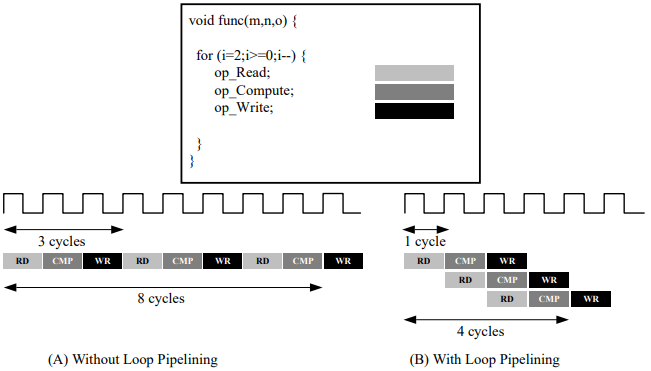
\includegraphics[width=1\textwidth]{solutions/loop_pipelining/looppipelining.png}
    \caption{HLS Loop Pipelining}
\end{figure}

In particolare, è possibile evidenziare due parametri fondamentali per questa tipologia di approccio:
\begin{itemize}
    \item \textbf{Iteration Latency (IL)}\\
    Numero di cicli che servono per eseguire un'iterazione del corpo del ciclo.
    \item \textbf{Initiation Interval (II) := Throughput}\\
    Numero di cicli di clock fino alla prossima iterazione del loop.
\end{itemize}

Idealmente, ci si aspetta un throughput pari a 1 perchè corrisponderebbe al caso migliore per il pipelining. Ovviamente non sempre è possibile ottenere un throughput pari a 1 ma in questo caso l'obiettivo è quello di ottenerlo.
\\
Il pipelining in HLS è possibile implementarlo mediante una direttiva proprietaria che permette, inoltre, di specificare l'Initiation Interval desiderato. Tanto è vero che all'interno del report di sintesi viene specificato l'II target, cioè quello specificato nella direttiva, e l'II raggiunto dal tool. Teoricamente, si dovrebbe ottenere II\_target=II\_achieved. Se così non fosse allora il tool non è riuscito a raggiungere l'obiettivo prefissato. Pertanto, si potrebbe modificare il codice per vedere se effettivamente il problema può essere risolto nella seguente maniera. Se così non fosse, evidentemente non dipende dal codice ma dal tipo di applicazione che si sta cercando di implementare che non lo permette.

\lstinputlisting[language=C++]{solutions/loop_pipelining/fir_loop_pipelining.cpp}

In questo caso, la soluzione hardware presa come riferimento è stata quella iniziale non ottimizzata. In particolare, all'interno del loop è stata definita sia la direttiva di pipeline, specificando un II=1, sia la direttiva di partizionamento. Nello specifico, è stato considerato il pragma di partitioning al fine di realizzabilità della soluzione in questione. Questo è dovuto al fatto che, senza considerare tale direttiva, si otterrebbe un II\_achieved differente da un II\_target. Infatti, utilizzare lo shift register vuol dire non poter accedere ai dati intermedi ma soltanto a quelli finali. Pertanto, per far fronte a questo problema si potrebbe pensare di realizzare tali shift register mediante Flip Flop (tramite la direttiva di partizionamento).
\\
Effettuando la sintesi otteniamo i seguenti report.

\begin{table}[H]
    \centering
    \begin{minipage}[t]{0.45\linewidth}
        \centering
        \begin{tabular}{|c|c|c|c|}
            \hline
            \textbf{Clock} & \textbf{Target} & \textbf{Estimated} & \textbf{Uncertainty} \\
            \hline
            ap\_clk & 10.00 & 8.510 & 1.25 \\
            \hline
        \end{tabular}
        \caption{HLS Loop Pipelining Solution Timing Summary (ns)}
        \label{tab:hls-loop-pipelining-solution-timing-summary}
    \end{minipage}
    \hfill
    \begin{minipage}[t]{0.45\linewidth}
        \centering
        \begin{tabular}{|c|c|c|c|}
            \hline
            \multicolumn{2}{|c|}{\textbf{Latency}} & \multicolumn{2}{|c|}{\textbf{Interval}} \\
            min & max & min & max \\
            \hline
            15 & 15 & 15 & 15 \\
            \hline
        \end{tabular}
        \caption{HLS Loop Pipelining Solution Latency Summary (clock cycles)}
        \label{tab:hls-loop-pipelining-solution-latency-summary}
    \end{minipage}
\end{table}

Si può notare come la latenza totale del loop sia notevolmente diminuita rispetto alla soluzione iniziale non ottimizzata. Inoltre, si può evidenziare come l'Initiation Interval raggiunto sia il medesimo di quello target, cioè pari a 1. Questo è stato possibile per i motivi precedentemente citati.
\\
In particolare, considerando il valore di Iteration Latency, il valore del Trip Count e il valore di Initiation Interval, è possibile ricavare il valore della latenza relativa al loop:
\begin{equation}
	IL+[(N-1)*II]-1 = 4+[(11-1)*1]-1 = 4+[10*1]-1 = 4+10-1 = 13	
\end{equation}

\begin{table}[H]
    \centering
    \begin{tabular}{|c|c|c|c|c|c|c|c|c|}
        \hline
        \multicolumn{1}{|c|}{Loop} & \multicolumn{2}{|c|}{\textbf{Latency}} & \multicolumn{2}{c|}{\textbf{Iteration Latency}} & \multicolumn{2}{c|}{\textbf{Initiation Interval}} & \multicolumn{1}{c|}{\textbf{Trip Count}}  \\
        Name & min & max & min & max & achieved & target &  \\
        \hline
        - loop & 13 & 13 & 4 & 4 & 1 & 1 & 11 \\
        \hline
    \end{tabular}
    \caption{HLS Loop Pipelining Solution Latency Loops Summary }
    \label{tab:hls-loop-pipelining-solution-loop-summary}
\end{table}

Per quanto riguarda l'utilizzazione stimata delle risorse, si può notare come il numero di FF sia aumentato rispetto alla soluzione non ottimizzata dal momento che è stato utilizzato il pragma di partizionamento tale da partizionare shiftRegister in diverse strutture da un certo numero di FF ciascuna anziché utilizzare BRAM.

\begin{table}[H]
    \centering
    \begin{tabular}{|l|c|c|c|c|}
        \hline
        \textbf{Name}    & \textbf{BRAM\_18K} & \textbf{DSP48E} & \textbf{FF} & \textbf{LUT} \\ \hline
        DSP              & -                   & -               & -           & -            \\ 
        Expression       & -                   & 4               & 0           & 480          \\ 
        FIFO             & -                   & -               & -           & -            \\ 
        Instance         & -                   & -               & -           & -            \\ 
        Memory           & 0                   & -               & 10          & 2            \\ 
        Multiplexer      & -                   & -               & -           & 75          \\ 
        Register         & -                   & -               & 700         & 64            \\ \hline
        \textbf{Total}   & 0                   & 4               & 710         & 621          \\ \hline
        \textbf{Available} & 280               & 220             & 106400      & 53200        \\ \hline
        \textbf{Utilization (\%)} & 0            & 1              & $\sim$0     & 1      \\ \hline
    \end{tabular}
    \caption{HLS Loop Pipelining Solution Utilization Estimates Summary}
    \label{tab:hls-loop-pipelining-solution-utilization-estimates-summary}
\end{table}

In particolare, si può notare come la direttiva proprietaria di partitioning ha partizionato shiftRegister in 10 strutture da 32 FF ciascuna.

\begin{table}[H]
	\centering
	\begin{tabular}{|l|r|r|r|r|}
		\hline
		\multicolumn{1}{|c|}{\textbf{Name}} & \multicolumn{1}{c|}{\textbf{FF}} & \multicolumn{1}{c|}{\textbf{LUT}} & \multicolumn{1}{c|}{\textbf{Bits}} & \multicolumn{1}{c|}{\textbf{Const Bits}} \\
		\hline
		accumulator\_reg\_114 & 32 & 0 & 32 & 0 \\
		ap\_CS\_fsm & 3 & 0 & 3 & 0 \\
		ap\_enable\_reg\_pp0\_iter0 & 1 & 0 & 1 & 0 \\
		ap\_enable\_reg\_pp0\_iter1 & 1 & 0 & 1 & 0 \\
		ap\_enable\_reg\_pp0\_iter2 & 1 & 0 & 1 & 0 \\
		ap\_enable\_reg\_pp0\_iter3 & 1 & 0 & 1 & 0 \\
		ap\_phi\_reg\_pp0\_iter1\_p\_pn\_reg\_138 & 32 & 0 & 32 & 0 \\
		ap\_phi\_reg\_pp0\_iter2\_p\_pn\_reg\_138 & 32 & 0 & 32 & 0 \\
		ap\_phi\_reg\_pp0\_iter3\_p\_pn\_reg\_138 & 32 & 0 & 32 & 0 \\
		coefficientsFilter1\_1\_reg\_458 & 10 & 0 & 10 & 0 \\
		i\_reg\_127 & 5 & 0 & 5 & 0 \\
		shiftRegister\_0 & 32 & 0 & 32 & 0 \\
		shiftRegister\_1 & 32 & 0 & 32 & 0 \\
		shiftRegister\_2 & 32 & 0 & 32 & 0 \\
		shiftRegister\_3 & 32 & 0 & 32 & 0 \\
		shiftRegister\_4 & 32 & 0 & 32 & 0 \\
		shiftRegister\_5 & 32 & 0 & 32 & 0 \\
		shiftRegister\_6 & 32 & 0 & 32 & 0 \\
		shiftRegister\_7 & 32 & 0 & 32 & 0 \\
		shiftRegister\_8 & 32 & 0 & 32 & 0 \\
		shiftRegister\_9 & 32 & 0 & 32 & 0 \\
		shiftRegister\_load\_p\_reg\_453 & 32 & 0 & 32 & 0 \\
		tmp\_1\_reg\_426 & 1 & 0 & 1 & 0 \\
		tmp\_2\_reg\_417 & 32 & 0 & 32 & 0 \\
		tmp\_4\_reg\_430 & 4 & 0 & 4 & 0 \\
		tmp\_6\_reg\_463 & 32 & 0 & 32 & 0 \\
		tmp\_reg\_422 & 1 & 0 & 1 & 0 \\
		tmp\_1\_reg\_426 & 64 & 32 & 1 & 0 \\
		tmp\_reg\_422 & 64 & 32 & 1 & 0 \\
		\hline
		Total & 700 & 64 & 574 & 0 \\
		\hline
	\end{tabular}
	\caption{HLS Loop Pipelining Solution Register Detail Estimates Summary}
	\label{tab:hls-loop-pipelining-solution-register-detail-estimates-summary}
\end{table}

Effettuando la C/RTL Cosimulation ed Export RTL si ottengono i seguenti report.

\begin{table}[H]
    \centering
    \begin{tabular}{|c|c|c|c|c|c|c|c|}
        \hline
        \multicolumn{1}{|c|}{RTL} & \multicolumn{1}{|c|}{Status} & \multicolumn{3}{c|}{\textbf{Latency}} & \multicolumn{3}{c|}{\textbf{Interval}} \\
        &  & min & avg & max & min & avg & max \\
        \hline
        VHDL & Pass & 15 & 15 & 16 & 15 & 15 & 16 \\
        \hline
    \end{tabular}
    \caption{HLS Loop Pipelining Solution C/RTL Cosimulation Summary }
    \label{tab:hls-loop-pipelining-solution-cosimulation-summary}
\end{table}

\begin{table}[H]
    \centering
    \begin{minipage}[t]{0.45\linewidth}
        \centering
        \begin{tabular}{|l|r|}
            \hline
            \textbf{Resource} & \textbf{VHDL} \\
            \hline
            SLICE & 204 \\
            \hline
            LUT & 311 \\
            \hline
            FF & 455 \\
            \hline
            DSP & 2 \\
            \hline
            BRAM & 0 \\
            \hline
            SRL & 0 \\
            \hline
        \end{tabular}
        \caption{HLS Loop Pipelining Solution Export RTL Resource Usage}
        \label{tab:hls-loop-pipelining-solution-export-rtl-resoruce-usage}
    \end{minipage}
    \hfill
    \begin{minipage}[t]{0.45\linewidth}
        \centering
        \begin{tabular}{|l|r|}
            \hline
            \textbf{Timing} & \textbf{VHDL} \\
            \hline
            CP required & 10.000 \\
            \hline
            CP achieved post-synthesis & 5.745 \\
            \hline
            CP achieved post-implementation & 6.512 \\
            \hline
        \end{tabular}
        \caption{HLS Loop Pipelining Solution Export RTL Final Timing}
        \label{tab:hls-loop-pipelining-solution-export-rtl-final-timing}
    \end{minipage}
\end{table}

Pertanto, importando l'IP in Vivado e impostando un clock constraint pari a 10ns è possibile analizzare i seguenti report di risorse, timing, potenza dinamica ed energia per singola operazione.
\lstinputlisting[language=VHDL]{solutions/loop_pipelining/clk_constraint.xdc}

Si può notare come, rispetto alla soluzione iniziale non ottimizzata, si è ottenuto un aumento di circa il $13\%$ delle LUT e un aumento di circa il $186\%$ dei FF.

\begin{table}[H]
    \centering
    \begin{tabular}{|c|c|c|c|c|c|c|}
        \hline
        \textbf{LUT} & \textbf{LUTRAM} & \textbf{FF} & \textbf{BRAM} & \textbf{DSP} & \textbf{IO} & \textbf{BUFG} \\
        \hline
        311 & 0 & 458 & 0 & 2 & 71 & 1 \\
        \hline
    \end{tabular}
    \caption{Vivado Loop Pipelining Solution Utilization Report [\#]}
    \label{tab:vivado-loop-pipelining-solution-utilization-report}
\end{table}

Inoltre, si può evidenziare come la maximum clock frequency sia aumentata di circa $15 MHz$ rispetto alla soluzione non ottimizzata di riferimento. Tanto è vero che il WNS, relativo alla soluzione realizzata mediante approccio di pipelining, risulta essere leggermente maggiore.

\begin{table}[H]
    \centering
    \begin{tabular}{|c|c|c|c|}
        \hline
        \textbf{Cycles} [\#] & \textbf{Clock Constraint} [ns] & \textbf{WNS} [ns] & \textbf{Maximum Clock Frequency} [Mhz] \\
        \hline
        16 & 10 & 4.208 & 172.6519337 \\
        \hline
    \end{tabular}
    \caption{Vivado Loop Pipelining Solution Timing Report}
    \label{tab:vivado-loop-pipelining-solution-timing-report}
\end{table}

In particolare, si può notare come, rispetto alla soluzione hardware iniziale non ottimizzata, i contributi di potenza dinamica sono aumentati tale da far aumentare l'energia per singola operazione. Nello specifico, si ha un aumento del contributo \textit{Clocks} di circa il $46\%$ dovuto principalmente all'aumento delle risorse associato alla solution in questione.

\begin{table}[H]
    \centering
    \begin{tabular}{|c|c|c|c|c|c|c|}
        \hline
        \textbf{BRAM} & \textbf{Clock Enable} & \textbf{Clocks} & \textbf{DSP} & \textbf{Logic} & \textbf{Set/Reset} [mW] & \textbf{Data} \\
        \hline
        0 & 0.196236724 & 1.778833685 & 0.814738101 & 1.275097136 & 0.012051522 & 1.206569896 \\
        \hline
    \end{tabular}
    \caption{Vivado Loop Pipelining Solution Dynamic Power Report [mW]}
    \label{tab:vivado-loop-pipelining-solution-dynamic-power-report}
\end{table}

\begin{table}[H]
    \centering
    \begin{minipage}[t]{0.45\linewidth}
        \centering
        \begin{tabular}{|c|}
            \hline
            \textbf{Dynamic Total} \\
            \hline
            5.283527065 \\
            \hline
        \end{tabular}
        \caption{Vivado Loop Pipelining Solution Dynamic Power Report [mW]}
        \label{tab:vivado-loop-pipelining-solution-total-dynamic-power-report}
    \end{minipage}
    \hfill
    \centering
    \begin{minipage}[t]{0.45\linewidth}
        \centering
        \begin{tabular}{|c|}
            \hline
            \textbf{Energy Single Operation} \\
            \hline
            52.83527065 \\
            \hline
        \end{tabular}
        \caption{Vivado Loop Pipelining Solution Energy Single Operation Report [pJ]}
        \label{tab:vivado-loop-pipelining-solution-energy-single-operation-report}
    \end{minipage}
\end{table}